\documentclass[11pt,a4paper]{article}
\usepackage[utf8]{inputenc}
\usepackage{amsmath}
\usepackage{amsfonts}
\usepackage{amssymb}
\usepackage{graphicx}
\usepackage{enumitem}

\usepackage{listings}
\lstdefinelanguage{scala}{
  morekeywords={abstract,case,catch,class,def,%
    do,else,extends,false,final,finally,%
    for,if,implicit,import,match,mixin,%
    new,null,object,override,package,%
    private,protected,requires,return,sealed,%
    super,this,throw,trait,true,try,%
    type,val,var,while,with,yield, synchronized},
  otherkeywords={=>,<-,<\%,<:,>:,\#,@},
  sensitive=true,
  morecomment=[l]{//},
  morecomment=[n]{/*}{*/},
  morestring=[b]",
  morestring=[b]',
  morestring=[b]"""
}

\usepackage{color}
\definecolor{dkgreen}{rgb}{0,0.6,0}
\definecolor{gray}{rgb}{0.5,0.5,0.5}
\definecolor{mauve}{rgb}{0.58,0,0.82}
\lstset{frame=tb,
  language=scala,
  aboveskip=3mm,
  belowskip=3mm,
  showstringspaces=false,
  columns=flexible,
  basicstyle={\small\ttfamily},
  numbers=none,
  numberstyle=\tiny\color{gray},
  keywordstyle=\color{blue},
  commentstyle=\color{dkgreen},
  stringstyle=\color{mauve},
  frame=single,
  breaklines=true,
  breakatwhitespace=true
  tabsize=3
}

\title{Semester project -- Pong Designer\\Technical report}
\author{\textit{Author:} Lomig Mégard\\
\textit{Supervisors:} Prof. Viktor Kuncak and Mikaël Mayer\vspace*{0.5cm}\\
\textsc{LARA/EPFL}}

\begin{document}
\maketitle

\section{Introduction}
This report explains de different implementation choices taken during the semester. The reader should first read the theoretical report in order to have the context.


\section{Type system}
The type system relies on type classes in Scala. For example, the signature of a property restrains the generic type that can be used.
\begin{lstlisting}
abstract class Property[T : PongType](...) {}
\end{lstlisting}

The \texttt{PongType} is defined in such a way we can translate an internal result of the interpreter to a Scala object, and the other way around.
\begin{lstlisting}
trait PongType[T] {
  def getPongType: Type
  def toPongValue(v: Any): Value
  def toScalaValue(v: Value): T
  def clone(v: T): T
}
\end{lstlisting}

The following method illustrates how these types can be used. The \texttt{Context} contains some global information required for the evaluation, as for example the current finger movements.
\begin{lstlisting}
def typecheckAndEvaluate[T : PongType](e: Expr): T = {
  typeCheck(e, implicitly[PongType[T]].getPongType)
  eval(e)(Context).as[T]
}
\end{lstlisting}

\section{Expressions and statements}
The AST of statements is illustrated in figure \ref{fig:AST-stats}. All classes are immutable but can reference a property whom value can change. Statements can have side-effect, here modifying a property value with the \texttt{Assign} operation. 

\begin{figure*}[h]
\centering
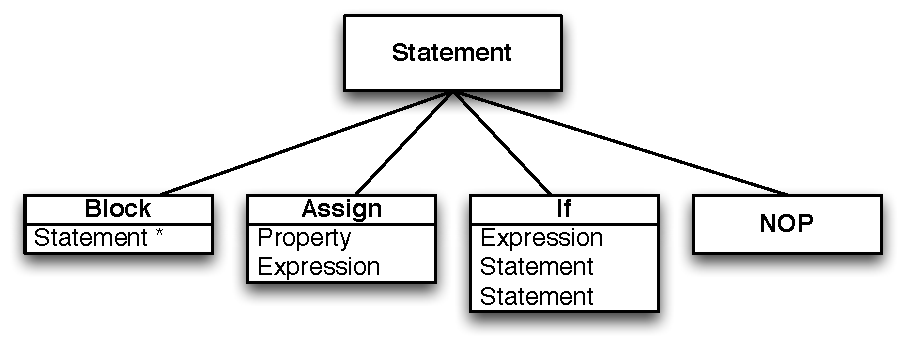
\includegraphics[scale = 0.7]{images/AST_stats} 
\caption{AST of statements.}
\label{fig:AST-stats}
\end{figure*}

The expressions cannot have side-effects. Here is a summarized list of the different kinds of expressions. The different expressions that use finger position and objects collision need a context to be evaluated. It is provided by the game engine that exposes the asynchronous events of the last terminated time step.
\begin{itemize}[noitemsep,topsep=2pt,parsep=1pt,partopsep=1pt]
\item Literals: \texttt{IntegerLiteral}, \texttt{StringLiteral}, ...
\item Arithmetic: \texttt{Add}, \texttt{Minus}, \texttt{Mod}, ...
\item Boolean: \texttt{And}, \texttt{LessThan}, \texttt{Equals}, ...
\item Finger: \texttt{MoveOver}, \texttt{DownOn}, ...
\item Collision
\item Property
\end{itemize}

\section{Game objects}
This project uses JBox2D version 2.2.1.1 for its physical engine. Since Pong Designer needs to handle the history of all properties, a wrapper named \texttt{PhysicalObject} is built around each JBox2D body. It takes care of instantiating the body with arbitrary expressions in the world and of managing the different properties with their history. 

\begin{figure*}[h]
\centering
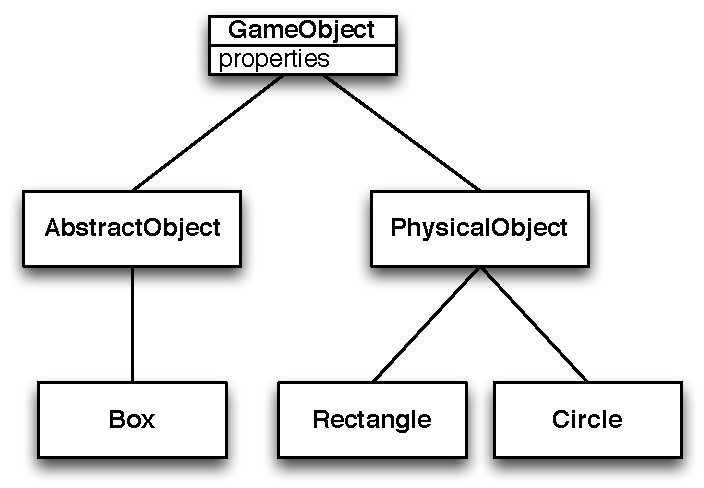
\includegraphics[scale = 0.7]{images/objects} 
\caption{Hierarchy of game objects.}
\label{fig:objects}
\end{figure*}

The figure \ref{fig:objects} describes how different kinds of game objects inherit from the same trait \texttt{GameObject}. It manages all the properties that belong to its implementation in two ways. First, each property is a class member of \texttt{GameObject} or of another sub-class if it is specific (an example is the circle radius). These members can be accessed only from the game engine itself, not from the user. This permits to have internally the right static Scala type for each property. Secondly, a map stores all the properties, even the ones declared in sub-classes, with their name for key. This enables the user to have access to a property from a name, but the precise type will remain unknown (it is anyway not required by the user). The following example shows how we can build a statement to increment a value.

\begin{lstlisting}
circle("x") := circle("x") + 1
\end{lstlisting}

This syntax is not very convenient but we assumed that this code would be generated by the game engine. It remains readable and meaningful.


\section{Categories of objects}

// Explain how categories are implemented

\begin{lstlisting}
foreach(cat) { o =>
  whenever(base("y") < o("y")) { Seq(
    o("y") := 0
  )}
}

foreach(cat1, cat2) { (o1, o2) =>
  once(Collision(o1, o2)) { Seq(
    score("value") += 1
  )}  
}
\end{lstlisting}


\section{Time management}
To manage a bounded history with good performances, I implemented a \texttt{RingBuffer} collection. It permits to have a complexity in $O(1)$ for \texttt{append}, \texttt{head} and \texttt{last} among others.

\section{Game loop}

\subsection{Time step}
The game loop uses fixed time step. The following code corresponds to the main loop that calls \texttt{update} and \texttt{render} on the game engine. The \texttt{update} call is redirected on the game itself if it is running.

\begin{lstlisting}
var canvas: Canvas = null
while(running) {
  canvas = null
  try {
    canvas = holder.lockCanvas()
    holder.synchronized {
      val beginTime = System.currentTimeMillis()
      var framesSkipped = 0

      // the view is the main game engine class
      view.update()
      view.render(canvas)

      val timeDiff = System.currentTimeMillis() - beginTime
      var sleepTime = FRAME_PERIOD - timeDiff

      if (sleepTime > 0) Try {
        Thread.sleep(sleepTime.toLong)
      }

      while (sleepTime < 0 && framesSkipped < MAX_FRAMES_SKIPPED) {
        // we missed a frame
        view.update()
        sleepTime += FRAME_PERIOD
        framesSkipped += 1
      }
    }
  } finally {
    if (canvas != null) holder.unlockCanvasAndPost(canvas)
  }
}
\end{lstlisting}


\subsection{Update}
The \texttt{update} method in the game follows a strict sequence of operations:
\begin{enumerate}
\item Evaluate the rules. The context can be used and contains all asynchronous events recorded since the last iteration. The collisions of the last physical step are also available.
\item Properties with new values are flushed to the physics engine.
\item Update the physical world using JBox2D. This performs new collisions and moves the objects.
\item Load new values from the physics engine to the properties.
\item Save the current state in the history.
\end{enumerate}








\end{document}
